
%%%%%%%%%%%%%%%%%%%%%%%%%%%%%%%%%%%%%%%%%%%%%%%%%%%%%%%%%%%%%%%%%%%%%%%%
%    INSTITUTE OF PHYSICS PUBLISHING                                   %
%                                                                      %
%   `Preparing an article for publication in an Institute of Physics   %
%    Publishing journal using LaTeX'                                   %
%                                                                      %
%    LaTeX source code `ioplau2e.tex' used to generate `author         %
%    guidelines', the documentation explaining and demonstrating use   %
%    of the Institute of Physics Publishing LaTeX preprint files       %
%    `iopart.cls, iopart12.clo and iopart10.clo'.                      %
%                                                                      %
%    `ioplau2e.tex' itself uses LaTeX with `iopart.cls'                %
%                                                                      %
%%%%%%%%%%%%%%%%%%%%%%%%%%%%%%%%%%
%
%
% First we have a character check
%
% ! exclamation mark    " double quote  
% # hash                ` opening quote (grave)
% & ampersand           ' closing quote (acute)
% $ dollar              % percent       
% ( open parenthesis    ) close paren.  
% - hyphen              = equals sign
% | vertical bar        ~ tilde         
% @ at sign             _ underscore
% { open curly brace    } close curly   
% [ open square         ] close square bracket
% + plus sign           ; semi-colon    
% * asterisk            : colon
% < open angle bracket  > close angle   
% , comma               . full stop
% ? question mark       / forward slash 
% \ backslash           ^ circumflex
%
% ABCDEFGHIJKLMNOPQRSTUVWXYZ 
% abcdefghijklmnopqrstuvwxyz 
% 1234567890
%
%%%%%%%%%%%%%%%%%%%%%%%%%%%%%%%%%%%%%%%%%%%%%%%%%%%%%%%%%%%%%%%%%%%
%
%%novalidate

\documentclass[12pt,a4paper,final]{iopart}
\newcommand{\gguide}{{\it Preparing graphics for IOP journals}}
%Uncomment next line if AMS fonts required
\usepackage{iopams}  
\usepackage{graphicx}
%\usepackage{amsmath}
%\usepackage{array}
\usepackage{enumitem}
\usepackage{multirow}
\usepackage{mathptmx}
\usepackage{longtable}
\usepackage[breaklinks=true,colorlinks=true,linkcolor=black,urlcolor=black,citecolor=black]{hyperref}
\usepackage[small,bf,singlelinecheck=on,labelformat=simple, labelsep=period]{caption}

\begin{document}

\title[Preparing an article for INCITEST 2020]{Application of Supply Chain Management Information System of Inventory at Computer Shop in Jambi City}

\author{Ade Indra Saputra$^{1*}$, Rahma Wahdiniwaty$^{2}$}
%\author{Ade Indra Saputra, Rahma Wahdiniwaty}
\address{$^1$Master of Information System Study, Postgraduate Faculty, Universitas Komputer Indonesia}
\address{$^2$Master of Management Study, Postgraduate Faculty, Universitas Komputer Indonesia}
%\address{$^2$Address Two, Neverland}
%\address{$^2$Universitas Komputer Indonesia}
\ead{ade.75118017@mahasiswa.unikom.ac.id}

%\author{Author Two}
%\address{Address Three, Neverland}
%\ead{author.two@mail.com}

%\author[cor1]{Author Three}
%\address{Address Four, Neverland}
%\eads{\mailto{author.three@mail.com}, %\mailto{author.three@gmail.com}}


\begin{abstract}
This study discusses the inventory system in requires good inventory management in order to manage the procurement for customers. Based on purpose of the study the make observations on the research by one of method approach that can be used in the management of the inventory is a method of Supply Chain Management (SCM)  concept for inventory control proccess. In inventory managing, the store needs a system that can ensure the supply of products in guranteed quality, on time delivery and the right amount in accordance with the reservation. By application of the supply chain management in calculate reorder point with safety stock can help control inventory in maintaining stock stability in improving customer service. Following the total reorder with saftey stock provides the effect to imporve business performance because it can improve the services to customers, sell new products, and increase sales. So, The XYZ Store can be estimated and predicted capital that must be spent every year, estimated revenue for the store and is able to maintain stability from stock out.

%The XYZ Store is a one of computer shop in Jambi City which selling computer equipment. This computer shop requires good inventory management in order to manage the procurement for customers precisely, estimated number of minimum ordered and predicted capital that must spent every year. So, a computerized system which is supported by supporting methods which chose in the prepartory proccess in computer shop to ensure that supplies can be existing. One of method that can be used in the management of the inventory is a method of Supply Chain Management (SCM). The system developed is a computer equipment inventory information system using the concept of Supply Chain Management use some software like MySQL for DBMS (Database Mangament System) and Web Application for selling in computer shop.

\end{abstract}

%Uncomment for PACS numbers title message
%\pacs{00.00, 20.00, 42.10}
% Keywords required only for MST, PB, PMB, PM, JOA, JOB? 
\vspace{2pc}
\noindent{\it Keywords}: SCM, Information System, Inventory
% Uncomment for Submitted to journal title message
%\submitto{\JPA}
% Comment out if separate title page not required
%\maketitle

\section{Introduction}

Competition between companies lately does not only occur in domestic companies, but also occurs globally as a result of the era of globalization and ASEAN free trade on Indonesia. The competition requires companies to provide the best service to consumers by ensuring the product distribution process up to the hands of consumers goes well. Various activities in production include activities to obtain raw materials, process them with various transformation processes become final products and distributed to consumers. Companies compete to meet the desires of consumers with "customer oriented" services, covering 3 main points namely price, quality, service (speed, comfort, etc.) \cite{Indrajit2016a}.

XYZ Store is a computer store that sells computer hardware and accesorries in Jambi. This company has to improve the quality of services to customers, by implementing appropriate strategies to win the competitions. Interview and observation data show this company often occurs out of stock in every month. High demand for goods, causing frequently out of stock and became unfulfilled orders. The Current web-based Transaction Processing system has been operated but did not have a stock management feature, and they cannot estimate the amount of goods should be purchased in the next month.

Estimates for inventory are usually predicted based on product items and the number of units sold. This technique is less effective, it is proven that there is a buildup of goods because it is not in accordance with the needs of the customer, plus the delay in the supply of goods causes a vacuum of goods which results in customer disappointment, and turns to the competitor's company. Product circulation is not running well and has an impact on customer service quality.

To overcome this problem, the authors designed the application to support XYZ Store business growth with features that can ensure that orders can be fulfilled, using the Supply Chain Management (SCM) method. The supply chain consists of all stages involved, directly or indirectly, in meeting customer demand. The supply chain includes not only producers and suppliers, but also transporters, warehouses, retailers, and customers themselves \cite{Sharma2012}.

SCM is needed for organizations to compete in dynamic international markets. The purpose of SCM is to combine internal activities and cross-organizational activities to provide customers value \cite{Habib2019}. Supply chain management is a form of competitive excellence which is applied in every industrial system \cite{Sampouw}. All these problems can be solved by the Supply Chain Management (SCM) approach which is an integrative method or approach that manages the flow of products, information, and money in an integrated manner involving parties ranging from upstream to downstream consisting of suppliers, factories, distribution networks, and logistics services \cite{Widianty2019}.

\section{Method}
\subsection{Data Collection Methodology and Data Analysis}
Data collection techniques began with observing business processes, interviews with owners and literature studies. Literature study is done by digging more information from similar research.

Data analysis was performed with qualitative and quantitative descriptive analysis. Qualitative descriptive analysis describes the relationship between supply chain management from the purchase and sale of products to customers. Quantitative descriptive analysis is performed to calculate the stock in the database from the initial inventory and ending inventory.

\subsection{Supply Chain Management Concept}

Supply Chain Management Professionals is Supply chain management encompasses the planning and management of all activities involved in sourcing, procurement, conversion, and all logistics management activities \cite{Liu2011a}. Encompasses the planning on business proccess management be a important to stores for the capitals management, it also includes the coordination and collaboration with channel partners, which can be suppliers, intermediaries, third-party service providers, and customers.

Guided by an integrated production plan, supported by various technologies, especially based on Internet/Intranet, and is implemented around supply, production operations, logistics (mainly manufacturing processes), and meeting demand which is Supply Chain Management \cite{Li2018}. Stated that supply chain is the network of companies that work hand-in-hand to create and deliver product to the hands of end users \cite{Sampouw}. W. Edwards Deming, author and consultant on quality, says that "The consumer is the most important part of the production line. Quality should be aimed at the needs of the consumer, present and future." \cite{Rusell2011}

\subsection{Evolution of Supply Chain Management}
The supply chain literature review was conducted to study the past researches. The emergence and evolution of SCM may be depicted as a timeline shown in \textbf{Figure \ref{figureEvolution}} \cite{Habib2019}.

\begin{figure}[htb!]
	\centering
	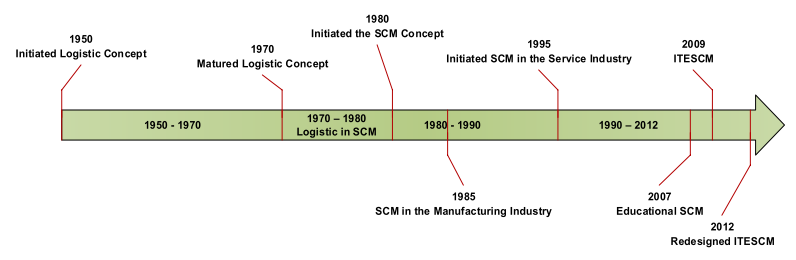
\includegraphics[width=1.0\textwidth]
		{evolution.png}
	\caption{\label{figureEvolution}Evolutionary Timeline of Supply Chain Management.}
\end{figure}

\subsection{Supply Chain Management Information System (SCM IS)}
The difference between companies between other companies is how to manage management information systems. So, In this modern era how companies manage their information will be the key to the success of a business failure \cite{Indrajit2016a}. Information systems are increasingly in supply chain management because of their ability to reduce costs and increase readiness in the supply chain \cite{Harianja2009}. Intensive information is needed in practice and innovative, so that the information system support is needed in an effective SCM and business strategy. This study, therefore, is at intersection of three important disciplines shown in \textbf{Figure \ref{figureScope}} \cite{Sathasivam, Harianja2009}.
\begin{figure}[htb!]
	\centering
	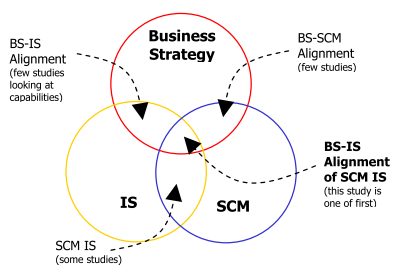
\includegraphics[width=0.5\textwidth]
	{scopeofstudy.png}
	\caption{\label{figureScope}Scope of Study. SCM IS Concept and Business Strategy.}
\end{figure}

\subsection{Lot Sizing Method}

In inventory control proccess there are several methods lotting that use. Lotting proccess is a proccess to determine the size of individual order that optimal based on calcuate result clean needs \cite{Ibrahim}. The use of the Lot Sizing technique is appropriate for use in determining the quantity of inventory orders in which in addition to minimizing the number of orders, it can also minimize the cost of direct inventory and inverse cost of inventory orders \cite{Djunaidi2019}. An inventory system controls the level of inventory by determining how much to order (the level of replenishment) and when to order. There are two basic types of inventory systems: a continuous (or fixed-order-quantity) system and a periodic (or fixed-time-period) \cite{Rusell2011}. 

%The several lot sizing method this following:\\
%\textbf{Lot Sizing MRP (Material Requirement Planning)} \cite{Almahdy}
%\begin{itemize}
%	\item Lot For Lot (LFL)\\
%	This technique is a lot sizing that most simple and easy to understand order placed with consider minimize saving costs.
%	\item Fixed Order Quantity (FOQ)\\
%	FOQ is stock system probabilistic that decision variable use Q (for Quantity) fixed order which optimal.
%	\item Economic Order Quantity (EOQ)\\
%	The function of the EOQ model is to determine the optimal order size that minimizes total inventory costs \cite{Rusell2011}.
%	\item Period Order Quantity (POQ)\\
%	POQ Technique is also called Economic Time Cycle. This technique use to determine time interval order (or Economic Order Interval).
%\end{itemize}

%Base on various research that lot sizing optimal method and economic is FOQ method because lowest total cost and have safety stock which is not too big \cite{Almahdy}. 

\subsection{Economic Order Quantity (EOQ)}
A formula for determining the optimal order size that minimizes the sum of carrying costs and ordering costs is the basic EOQ model \cite{Rusell2011}. The XYZ Store has unsold inventory, so the store has a carrying cost for the product.

Assumptions of case to model formula \cite{Rusell2011}: 
\begin{itemize}
	\item Demand is known with certainty and is constant over time.
	\item No shortages are allowed.
	\item Lead time for the receipt of orders is constant.
	\item The order quantity is received all at once.
\end{itemize}
This following is a formula of the basic EOQ, (\ref{rumusFOQ}) :

\begin{eqnarray}
	\label{rumusFOQ}
	Q_{opt} &= \sqrt{\frac{2C_oD}{C_c}}
\end{eqnarray}
where:\\
- Q$_{opt}$ = Quantity optimal (Economic Order Quantity)\\
- $C_o$ = Ordering cost every order\\
- D = Demand rate\\
- $C_c$ = Carrying cost/Holding cost

The total minimum cost is determined by substituting the value for the optimal order size, Q$_{opt}$, into the total cost equation (\ref{rumusMin}) :
\begin{eqnarray}
	\label{rumusMin}
	TC_{min} &= \frac{C_oD}{Q_{opt}} + \frac{C_cQ_{opt}}{2}
\end{eqnarray}

\subsection{Reorder Point (ROP)}
Reorder point is a point which is a new order have to do (or prepartions begin). This things influenced by lead time. Time to need for recieve order quantity after the order to made. This following to getting reorder point, (\ref{rumusROP}) \cite{Rusell2011}:
\begin{eqnarray}
	\label{rumusROP}
	R &= d \times L
\end{eqnarray}
where:\\
- d = demand rate per period (e.g., daily)\\
- L = lead time

\subsection{Safety Stock}
Safety stock an order is made when the inventory level reaches the reorder point. During the lead time the remaining inventory in stock will be depleted at a constant demand rate, such that the new order quantity will arrive at exactly the same moment as the inventory level reaches zero. While XYZ Store is met with uncertainty about demand so there will be a possibility of stock out. This following to getting reorder point with safety stock (\ref{rumusROPs}) \cite{Rusell2011}:
\begin{eqnarray}
	\label{rumusROPs}
	R &= \overline{d}L + z\sigma_d\sqrt{L}
\end{eqnarray}
where:\\
- $\overline{d}$ = average daily demand\\
- L = lead time\\
- $\sigma_d$ = the standard deviation of daily demand\\
- z = number of standard deviation corresponding to the service level probability\\
- z$\sigma_d\sqrt{L}$ = safety stock

\section{Results and discussion}
The results of the study were conducted experiments on data taken from sales applications. This following data product in store \textbf{Table \ref{tableBarang}} :
\begin{table}[h!]
	\centering
	\caption{\label{tableBarang} Data transaction popular in 2019 years old at xyz store}
	\begin{tabular}{ cllcl }
		\hline
		\textbf{Numb.} & \textbf{Code} & \textbf{Product Name} & \textbf{Annual Demand} & \textbf{Price} \\
		\hline
		1 & BRG037 & Cart 810 & 103 & Rp. 185.000,-  \\ 
		2 & BRG234 & Tinta alfa ink canon hitam 100 ML & 53 &  Rp. 28.500,-  \\ 
		3 & BRG038 & Cart 811 & 35 & Rp. 235.000,- \\ 
		\hline
	\end{tabular}
\end{table}

Base on table \ref{tableBarang} is the sales data obtained from the sales application in the XYZ store. While the number of sales per product can be seen in the following data:
\begin{center}
	\begin{longtable}{ clcc }
		\caption{\label{tableOut} Data stock out, product: Cart 810 in 2019 years old at xyz store}\\
		\hline
		\textbf{Numb.} & \textbf{Month} & \textbf{In} & \textbf{Out} \\
		\hline
		1 & January & 15 & 16  \\ 
		2 & February & 5 & 6  \\ 
		3 & March & 10 & 10 \\ 
		4 & April & 10 & 10 \\ 
		5 & May & 15 & 13 \\ 
		6 & Juny & 5 & 6 \\ 
		7 & July & 10 & 8 \\ 
		8 & August & 10 & 8 \\ 
		9 & September & 10 & 6 \\ 
		10 & October & 5 & 9 \\ 
		11 & November & 10 & 3 \\ 
		12 & December & 0 & 8 \\ 
		\hline
		\multicolumn{2}{c}{Total} & {105} & {103}\\
		\hline
	\end{longtable}
\end{center}

Based on the table \ref{tableOut} is sales and purchase data obtained from sales applications in XYZ stores based on Cartrige 810 products for a year.\\ \\
\textbf{Calculate EOQ Product: Cart (Cartrige) 810}
\begin{enumerate}[label=(\alph*)]
	\item Demand (D) = The estimate demand order product cart 810 in 2019 years old = 103 Pcs
	\item Order Cost ($C_o$) = The order cost every order = Rp. 15.000,-
	\item Unit Cost = Price cart 810 = Rp. 185.000,-
	\item Lead Time (L) = The lead time while an order made = 2 day
	\item Carying Cost ($C_c$) = Holding cost per unit 10\% from product price = (Heizer \& Render) (Rp. 185.000 $\times$ 10\%) = Rp. 18.500,-
\end{enumerate}
So, the optimal order size is if use formula (\ref{rumusFOQ}) :\\

$Q_{opt}$ = $\sqrt{\frac{2(Rp15.000)(103)}{Rp18.500}}$ = 13 Pcs\\ \\
The total annual inventory cost is determined by substituting $Q_{opt}$ into the total cost formula (\ref{rumusMin}):\\

$TC_{min}$ = $\frac{(Rp15.000)(103)}{13}$ + $\frac{(Rp18.500)(103)}{2}$\\

= Rp. 1.071.596,-\\ \\
The number of orders per year is computed as follows:

Number of orders per year = $\frac{D}{Q_{opt}}$

= $\frac{103}{13}$

= 8 order per year\\ \\
\textbf{Calculate Reorder Point (ROP): Cart 810}\\
The total reorder point by formula (\ref{rumusROP}) this following:
\begin{enumerate}[label=(\alph*)]
	\item Lead Time (L) = 2 day 
	\item The average using of product in a month = 103/12 = 8,5 (or 9) Pcs
	\item Estimate needed per day (d) = 9/20 (work day) = 0,45
\end{enumerate}

R = 0,45 $\times$ 2

= 0,9 (or 1) Pcs\\

So, the conclusion is when the product inventory reaches 1 Pcs, it must be ordered as many as 13 Pcs. For the possibility of shortages, this ROP model can be combined with Safety Stock, which is a stock reserve that must be held to avoid the shortage of goods, especially when waiting for goods that are being ordered. As a hedge against stockouts when demand is uncertain, a safety stock of inven- tory is frequently added to the expected demand during lead time \cite{Rusell2011}. The assumes demand during lead time follow a normal curve, just average and deviation standard that needed to describe inventory needed to increase service. The service level is the probability that the amount of inventory on hand during the lead time is sufficient to meet expected demand that is, the probability that a stock out will not occur \cite{Rusell2011}. A service level of 90\% mean that there is a 0.90 probability that demand will be met during the lead time and the probability that a stock out will occur is 10\% \cite{Rusell2011}.\\ \\
\textbf{Calculate Reorder Point with Safety Stock (ROPs): Cart 810}\\
This following the total reorder with safety stock by use formula (\ref{rumusROPs}) :

\begin{enumerate}[label=(\alph*)]
	\item The average daily demand per day ($\overline{d}$) = 1 Pcs per day
	\item Lead time (L) = 2 day
	\item standard deviation (z) = 3,44
\end{enumerate}

Safety Stock = z$\sigma_d\sqrt{L}$

= (3,44)(1)($\sqrt{2}$)

= 1,41 Pcs\\
The reorder point is computed as follows base on formula \ref{rumusROPs} add safety stock:

R = 0,9 + 1,41

= 2,31 Pcs\\
So, if when stock to reach 2 or 3 pcs, it must be reorder as many as 13 Pcs. In accordance with previous EOQ calculations.


\section{Conclusion}
By Using the EOQ model and supply chain management concept can help control inventory in maintaining stock stability in improving customer service. Then be able to maintain expenditure on holding costs and capital can be managed properly. The XYZ Stores make an order every month from the results of this study can be seen how many times a year to make an order. So, The XYZ Stores can be estimated and predicted capital that must be spent every year, estimated revenue for the store and is able to maintain stability from stock out.

\section*{Acknowledgments}
The authors would like to thank Mr. Prof. Dr. Ir. Eddy Soeryanto Soegoto, MT as Chancellor of the Universitas Komputer Indonesia (UNIKOM), Mrs. Dr. Rahma Wahdiniwaty, Dra., M.Si. as Dean of Postgraduate Faculty,  Mr. Dr. Yeffry Handoko Putra, ST., M.T. as Head of the Master of Information Systems, Mr. Mulyadi, S.Kom, M.S.I. Lecture of the Universitas Dinamika Bangsa (UNAMA) Jambi. And special thanks were given to Dr. Rahma Wahdiniwaty, Dra., M.Si. who have provided full support and guidance so that this paper can be realized. 


\section*{References}
\bibliographystyle{IEEEtran}
\bibliography{library}
%\begin{thebibliography}{10}
%\bibitem{ref1} J.~Doe, Article name, \textit{Phys. Rev. Lett.}

%\bibitem{ref2} J.~Doe, J. Smith, Other article name, \textit{Phys. Rev. Lett.}

%\bibitem{web} \href{http://www.google.pl}{www.google.pl}
%\end{thebibliography}

\end{document}

